\section{Recherche}

Im Zuge unserer Recherche haben wir beschlossen, uns grob an einem Plan von Nick Roethe für einen \glqq{}80m-1W-Fuchsjagdsender\grqq{} für unseren Aufbau zu orientieren.\\
\begin{figure}[H]
	\centering
	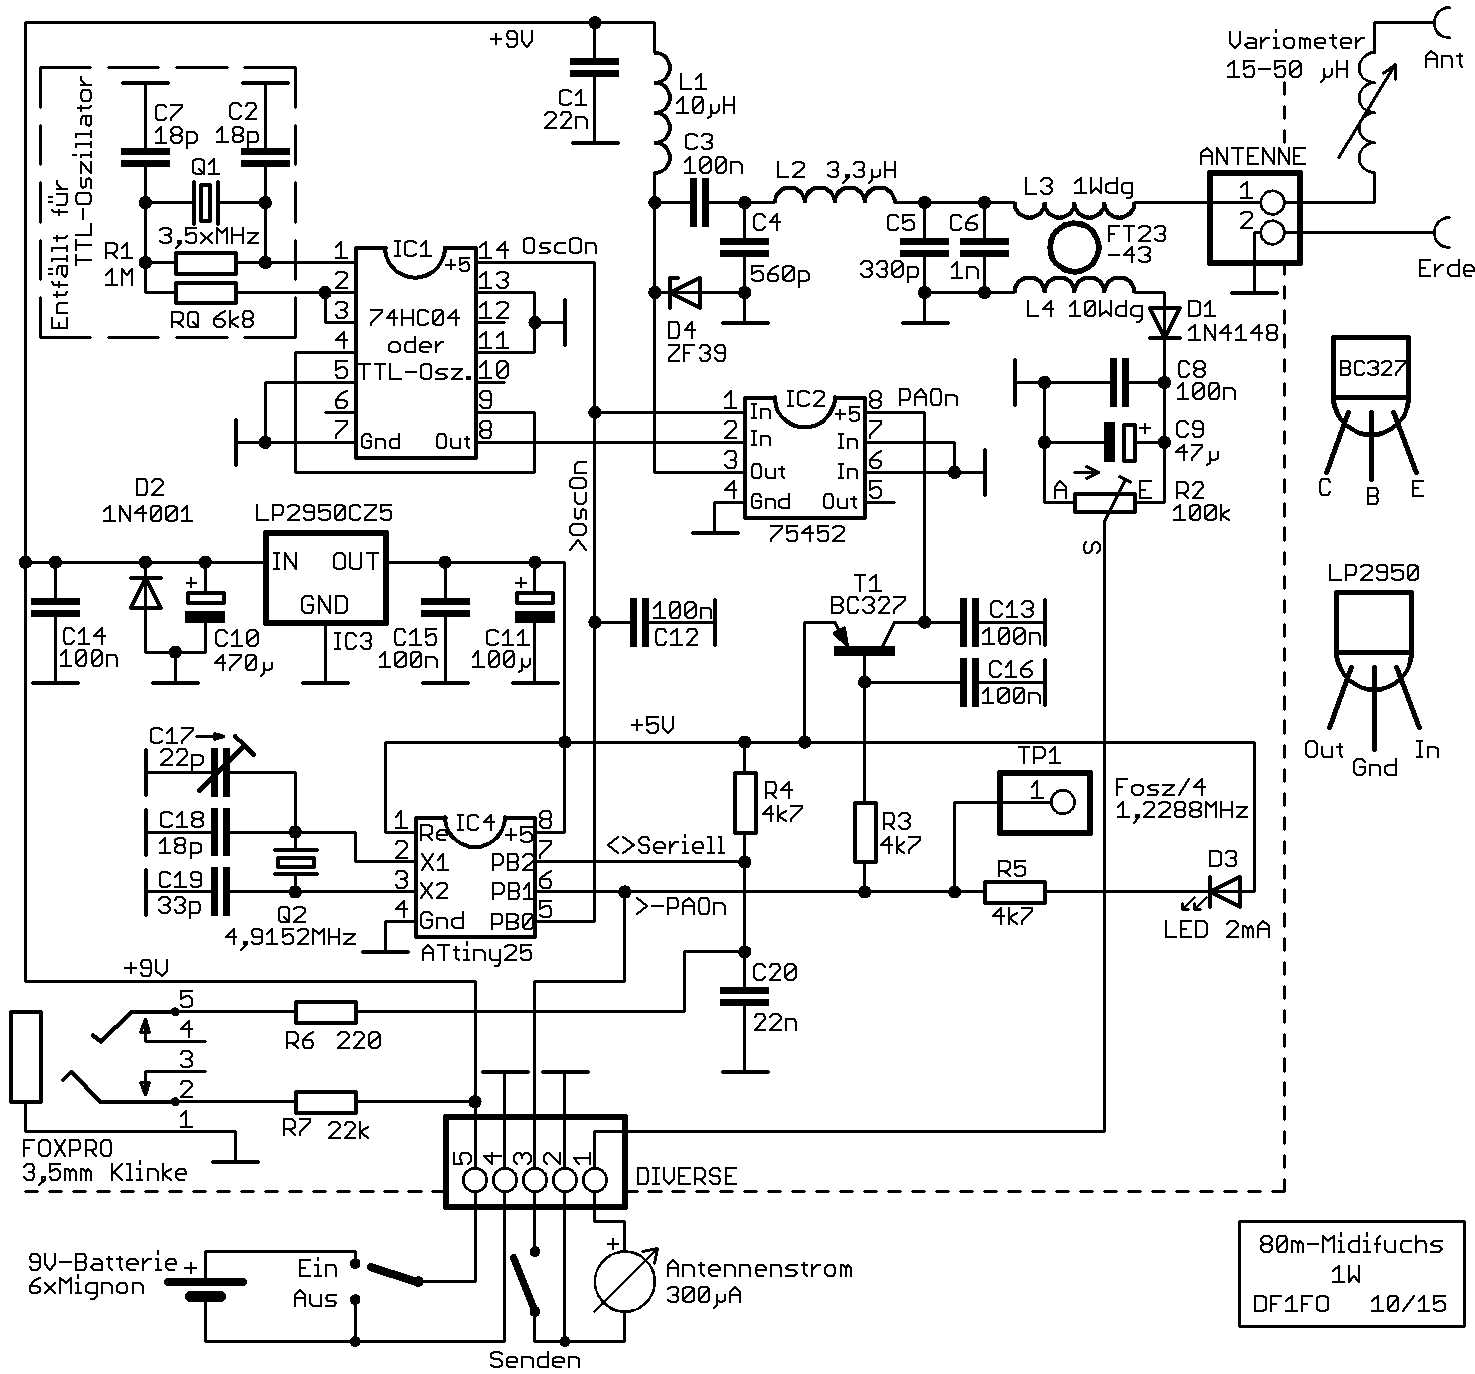
\includegraphics[width=16cm]{res/Recherche_Aufbau.png}
	\caption{Schaltung des Fuchsjagdsenders von Nick Roethe}
\end{figure}

Für die Wahl unserer Bauteile haben wir uns wo möglich für SMD-Bauteile entschieden wegen der kleineren Serieninduktivität der Kondensatoren und zur Platzersparnis.
Zum generieren des hochfrequenten Sendesignals bietet sich ein einfach zu verschaltender Quarzoszillator an, der nicht erst zum Schwingen angeregt werden muss. 
Indem wir für die Bedienung ein Potentiometer verwenden, das wir mit Hilfe eines DIP-Schalters umschalten, können wir am Mikrocontroller I/O-Pins sparen und so bei einem billigeren Modell bleiben. Zum takten des Mikrocontrollers ist es ratsam, den ohnehin vorhandenen und temperaturresistenteren Quarzoszillator zu verwenden, damit es nicht zu Abweichungen kommt, die während eines Wettbewerbs dazu führen könnten, dass sich Signale von verschiedenen Sendern überlappen. 
Um die Anforderungen bezüglich der Energieversorgung zu erfüllen sollten 3 Lithium-Polymer-Zellen mehr als ausreichen.\\
Da wir im 80-Meter-Band senden wollen, müsste die Antenne idealerweise 20m lang sein, aber wahrscheinlich wird die verwendete Antenne höchstens 10m lang werden und damit weit besser dafür geeignet sein, die erste Oberschwingung zu übertragen, die deshalb stärker gedämpft werden sollte. Die im Onlinehandel verfügbaren Spulen, die einen angemessenen Preis haben, weisen hohe Toleranzen von mindestens 10\% auf und die Auswahl ist begrenzt. Um die Induktivitäten, die für die Funktion des Filters ausschlaggebend sind, besser zu treffen, müssen wir die Spulen daher selbst wickeln.

%toDo: Fällt noch wem was ein?